\subsection{Module}
De module is de Haskell bibliotheek die de programmeur gebruikt om de grafische interface in de client te bedienen. Naar de programmeur is de gebruiksvriendelijkheid van de biblotheek een van de belangrijkste overwegingen voor het ontwerp. De module bestaat uit een aantal onderdelen: de server die de statische bestanden serveert, de websocket server die de verbinding met de client onderhoud, en de laag die de input en output verwerkt. \autoref{fig:architecture_module} geeft de architectuur weer van de module.

-TODO: Ontwerpkeuze toelichten: De server draait in het process van de studentcode

-TODO: Ontwerpkeuze toelichten: unsafePerformIO in Server.hs

\begin{figure}
\begin{center}
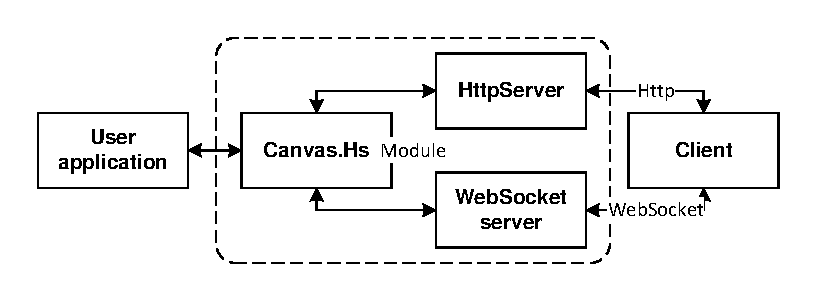
\includegraphics[keepaspectratio,width=\textwidth]{./images/module_architecture.pdf}
\caption{Architectuur van de module}
\label{fig:architecture_module}
\end{center}
\end{figure}


\paragraph{Gebruik} Wanneer de programmeur gebruik wil maken van de Canvas.hs moet hij gebruik maken van de installEventHandler functie. Bij het aanroepen van deze functie moet de programmeur een event handler meegeven die alle events vanuit de interface afhandeld. Om het gebruik van Canvas.hs zo makkelijk mogelijk te houden zal bij het aanroepen van installEventHandler automatisch de statische server en de websocket server gestart worden, en daarna automatisch de browserpagina geopend worden. \autoref{fig:startup_procedure} geeft de opstartprocedure weer.

\begin{figure}
\begin{center}
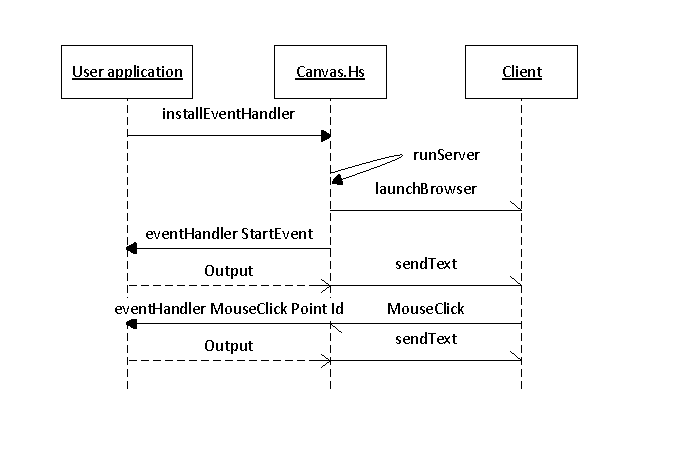
\includegraphics[keepaspectratio,width=\textwidth]{./images/module_startup_procedure_interaction.pdf}
\caption{De opstartprocedure en initiele interactiesequentie}
\label{fig:startup_procedure}
\end{center}
\end{figure}


\paragraph{Input/output}
De module handeld input en output af door events naar de eventhandler van de programmeur te sturen. Bijvoorbeeld: wanneer een gebruiker op een rondje klikt zal het programma de event handler aanroepen met de ID van dat rondje en de lokatie van de muisklik. De event handler van de programmeur kan dan nieuwe output genereren op basis van dit event. Zoals een nieuw menu weergeven of het uitvoeren van een actie zoals het opvragen van een bestand van de gebruiker.In \autoref{fig:startup_procedure} is deze interactie weergegeven. 

\paragraph{Servers}
Canvas.hs draait een simpele server op port 80 die statische bestanden kan serveren. Waaronder de index pagina, de javascript bestanden en eventueel plaatjes. Op port 8080 draait een websocket server die de verbinding met de client onderhoud.

